\documentclass[11pt,a4paper,twoside]{article}
\usepackage[dutch]{babel}
%laad de pakketten nodig om wiskunde weer te geven :
\usepackage{amsmath,amssymb,amsfonts,textcomp}
%laad de pakketten voor figuren :
\usepackage{graphicx}
\usepackage{float,flafter}
\usepackage{hyperref}
\usepackage{inputenc}
\usepackage{listings}
%zet de bladspiegel :
\setlength\paperwidth{20.999cm}\setlength\paperheight{29.699cm}\setlength\voffset{-1in}\setlength\hoffset{-1in}\setlength\topmargin{1.499cm}\setlength\headheight{12pt}\setlength\headsep{0cm}\setlength\footskip{1.131cm}\setlength\textheight{25cm}\setlength\oddsidemargin{2.499cm}\setlength\textwidth{16.5cm}

\begin{document}
\begin{center}
{\bf {\Huge UNIVERSITY OF VICTORIA} ~\\
	~\\
	{\huge Department of Electrical and Computer Engineering} ~\\
	~\\
	~\\
	{\huge ECE 403/503 Optimization for Machine Learning} ~\\
	~\\
	~\\
	~\\
	{\huge LABORATORY REPORT}
	~\\
	~\\
	~\\
}
\end{center}
{\bf
{\LARGE Experiment No: 01}
~\\
~\\
~\\
{\LARGE Title: Handwritten Digits Recognition Using PCA}
~\\
~\\
~\\
{\LARGE Date of Experiment: 28 May, 2019}
~\\
~\\
~\\
{\LARGE Report Submitted on: 4 June, 2019}
~\\
~\\
~\\
{\LARGE To: Mr. J. Zhan}
~\\
~\\
~\\
{\LARGE Laboratory Group No.: B01 T}
~\\
~\\
~\\
{\LARGE Name(s): Alvi Mahadi (V00912845)}
~\\
~\\
~\\
}

\newpage
% !TEX root = main.tex
\section{Introduction and Objectives}
\label{sect:introduction}
In this experiment, we investigate a technique for multi-category classification based on binary
classifications. The technique is then applied to Fisher`s 3-class datasets of Iris plants to
demonstrate its effectiveness. The dataset of Iris plants to be used in this experiment was created
and published in 1936 by R. A. Fisher [1]. Fisher's paper is a classic in the field and is referenced
frequently to this day, as a matter of fact the dataset is arguably the best-known in the pattern
recognition literature [2]. The dataset includes features of 150 Iris plants of 3 species known as
Setosa, Versicolor, and Virginica, where each sample Iris is represented by a 4-dimensional vector
in terms of lengths and widths of the sepal and petal of the flower.
% !TEX root = main.tex
\section{Implementation Steps and Results}
\label{sect:implementation-result}

\subsection{Implementation Steps}
\label{subsect:implementation_steps}
We strictly followed the implementation steps stated in the laboratory manual [3].

\subsection{Code}
\label{subsect:code}

\begin{lstlisting}[language=Matlab]
clc;
clear all;
close all;
D_tr = load('/home/alvi/Documents/courses/ece503/labs/3/data/D_build_tr.mat');
Xtr = D_tr.D_build_tr(1:8,:);
Ytr = D_tr.D_build_tr(9:10, :);
D_te = load('/home/alvi/Documents/courses/ece503/labs/3/data/D_build_te.mat');
Xte = D_te.D_build_te(1:8,:);
Yte = D_te.D_build_te(9:10, :);
Xtr = [Xtr' ones(640, 1)];
I = eye(9);
W_B = pinv(Xtr' * Xtr + 0.01 * I) * Xtr' * Ytr';
W = [W_B(1:8, 1) W_B(1:8, 2)];
b = W_B(9, :)';
e_p = double.empty();
Y = double.empty();
for i=1:128
y = W' * Xte(:, i) + b;
Y = [Y, y];
end
e_p = norm(Yte - Y, 'fro') / norm(Yte, 'fro');
disp(e_p);
I = 1:128;
plot(I, Yte(1, I), 'r', I, Y(1, I), 'g');
plot(I, Yte(2, I), 'r', I, Y(2, I), 'g');
\end{lstlisting}

\subsection{Result}
\label{subsect:result}
\begin{figure}[h]
	\centering
	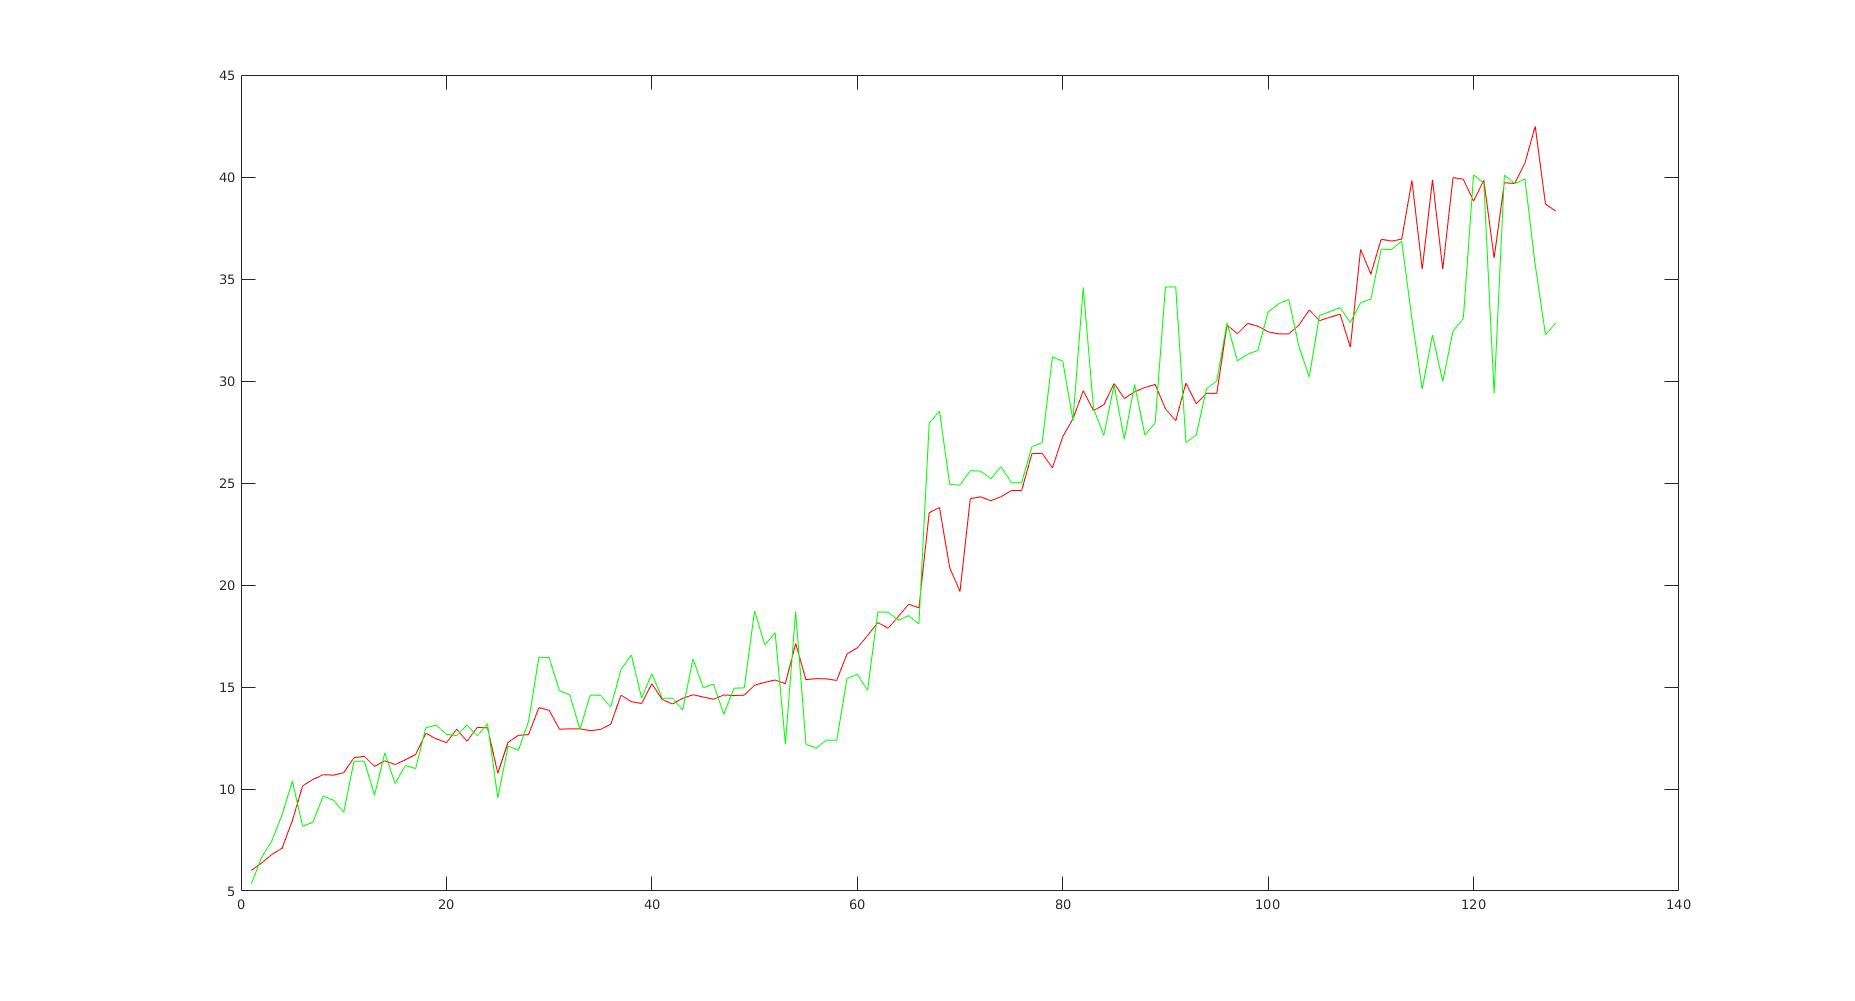
\includegraphics[width=\textwidth]{/home/alvi/Documents/courses/ece503/labs/3/result/1.jpg}
	\caption{First row of $Yte$ and first row of $Y^{(p)}$}
	\label{fig:1}
\end{figure}

\begin{figure}[h]
	\centering
	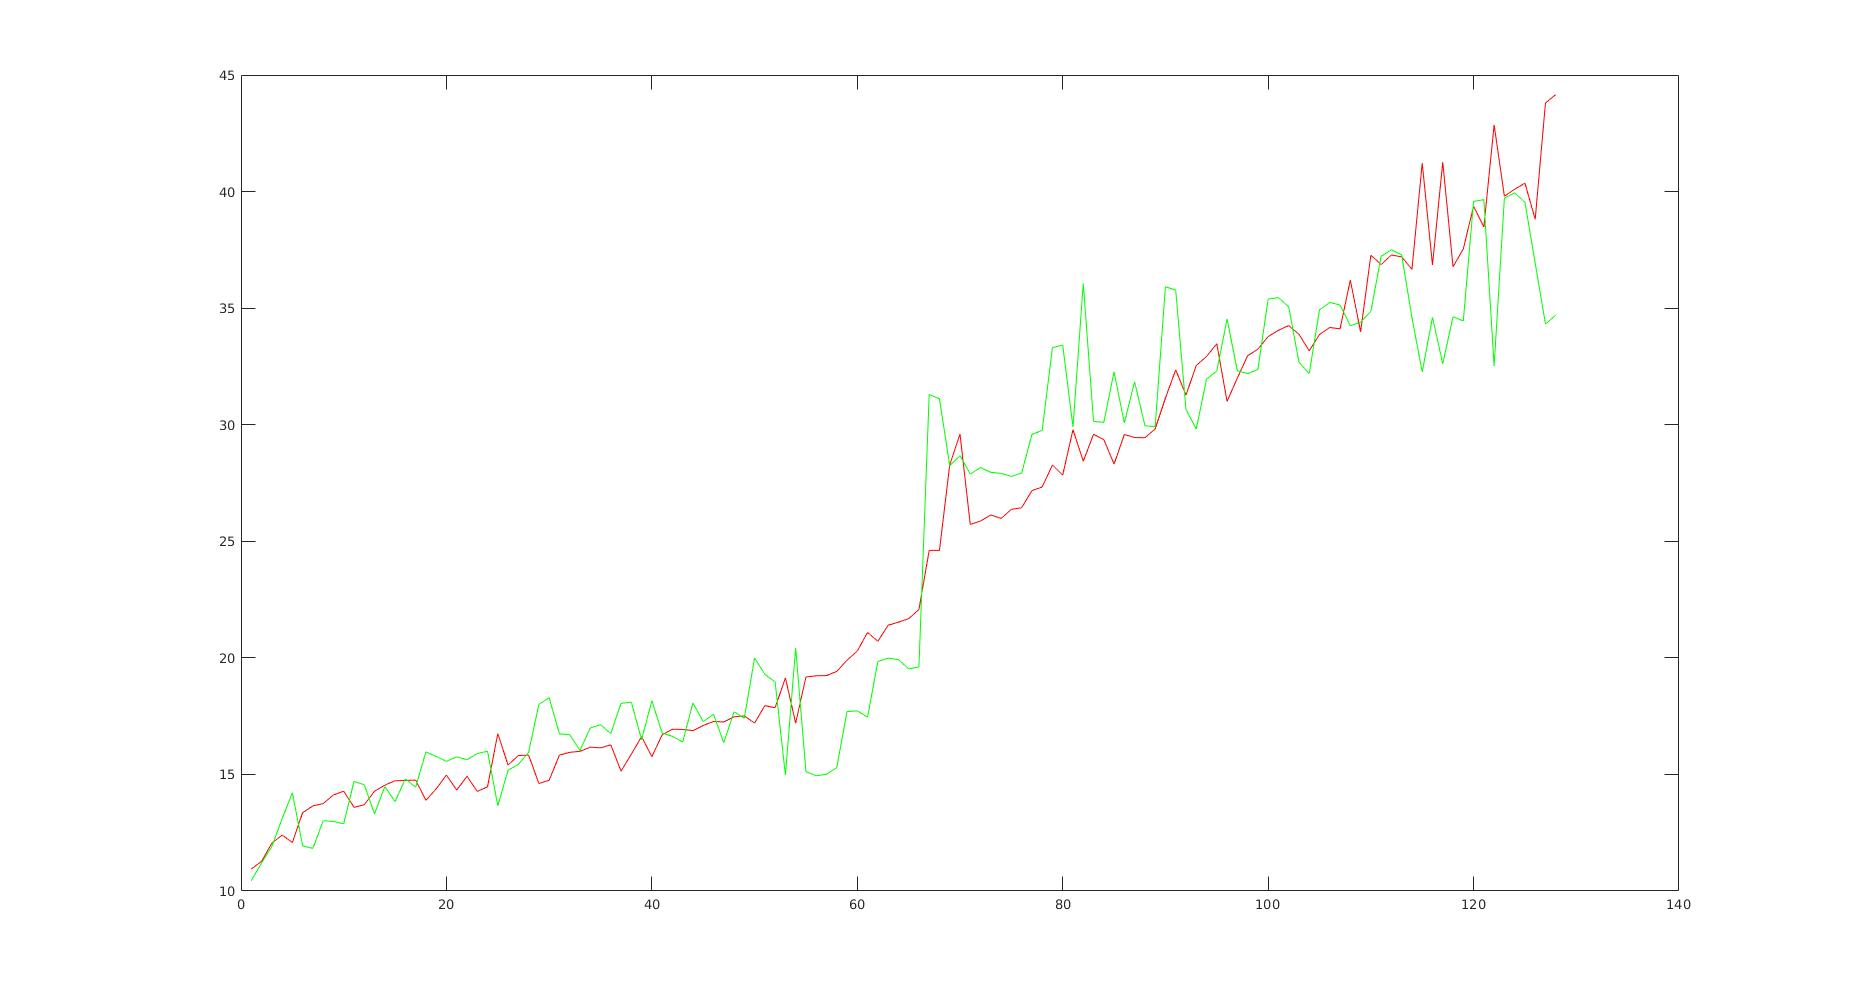
\includegraphics[width=\textwidth]{/home/alvi/Documents/courses/ece503/labs/3/result/2.jpg}
	\caption{Second row of $Yte$ and second row of $Y^{(p)}$}
	\label{fig:1}
\end{figure}
% !TEX root = main.tex
\section{Discussion}
\label{sect:discussion}
Fisher’s dataset is a matrix of size $5\times150$ whose first 4 rows are the data of the 150 samples, and the last row contains labels of the 150 flowers. The matrix D\_iris was constructed so that its first 50 columns are associated with Iris Setosa, the next 50 columns are for Iris Versicolor, and the last 50 columns are for Iris Virginica. For each data class of 50 samples, 40 samples are used for training and the remaining 10 samples are used for testing. Random selection of the samples is made for all three data classes as follows. 

After going through the process stated in section 3.3 in [3], we've found our confusion matrix as
\begin{verbatim}
29     1
1    29
\end{verbatim}
which essentially points that we have 29 out of 30 test cases as is classified True Positive, 1 out of 30 cases is classified as False Positive. The $12^{th}$ data which is actually ``Versicolor'' is classified as ``Verginica''. From the confusion matrix we can observe that, the Error Rate of our experiment is 0.03333 which is very accurate.
% !TEX root = main.tex
\section{Conclusion}
\label{sect:conclusion}
From our analysis we can see that PCA and Euclidean distance work well for the recognition of the hand digit characters. But the PCA was initially introduced for dimension reduction. We can see from our experiment that the dimension of our train dataset in reduced a great deal using PCA and it contributes to the high speed execution of our program resulting in under 1 sec per 1,000 characters. This result justifies our choice of using PCA as the feature extraction technique. There are a lot to be done in term of classifying the dataset. The accuracy of our analysis can be higher with some other classification techniques such as Support Vector Machine(SVM).

\section{References}
[1] R. A. Fisher, "The use of multiple measurements in taxonomic problems”, Annual Eugenics,
vol. 7, part II, pp. 179-188, 1936. \\\relax
[2] UCI Machine Learning, http://archive.ics.uci.edu/ml, University of California Irvine, School of
Information and Computer Science. \\\relax
[3] LABORATORY MANUAL, ECE 403/503 - OPTIMIZATION for MACHINE LEARNING, Prepared by: Wu-Sheng Lu, Department of Electrical and Computer Engineering, University of Victoria.
   
\end{document}